\documentclass[main.tex]{subfiles}
\newcommand\chapterlabel{Ch-electrochem}\setcounter{figurenewcounter}{0}\setcounter{tablenewcounter}{0}\setcounter{formulanewcounter}{0}\chapterpicture{../{\chapterlabel}/figure1}\chapterpicturelabel{PxFuel}
\setcounter{figurenewcounter}{0}





\begin{document}
%\linenumbers
%\setcounter{chapter}{5}
  
 \setcounter{chapter}{8}  \import{../\chapterlabel/files/}{ChapterName}


%      \begin{marginfigure}
%      \begin{tikzpicture} \node (a) at (0,0) {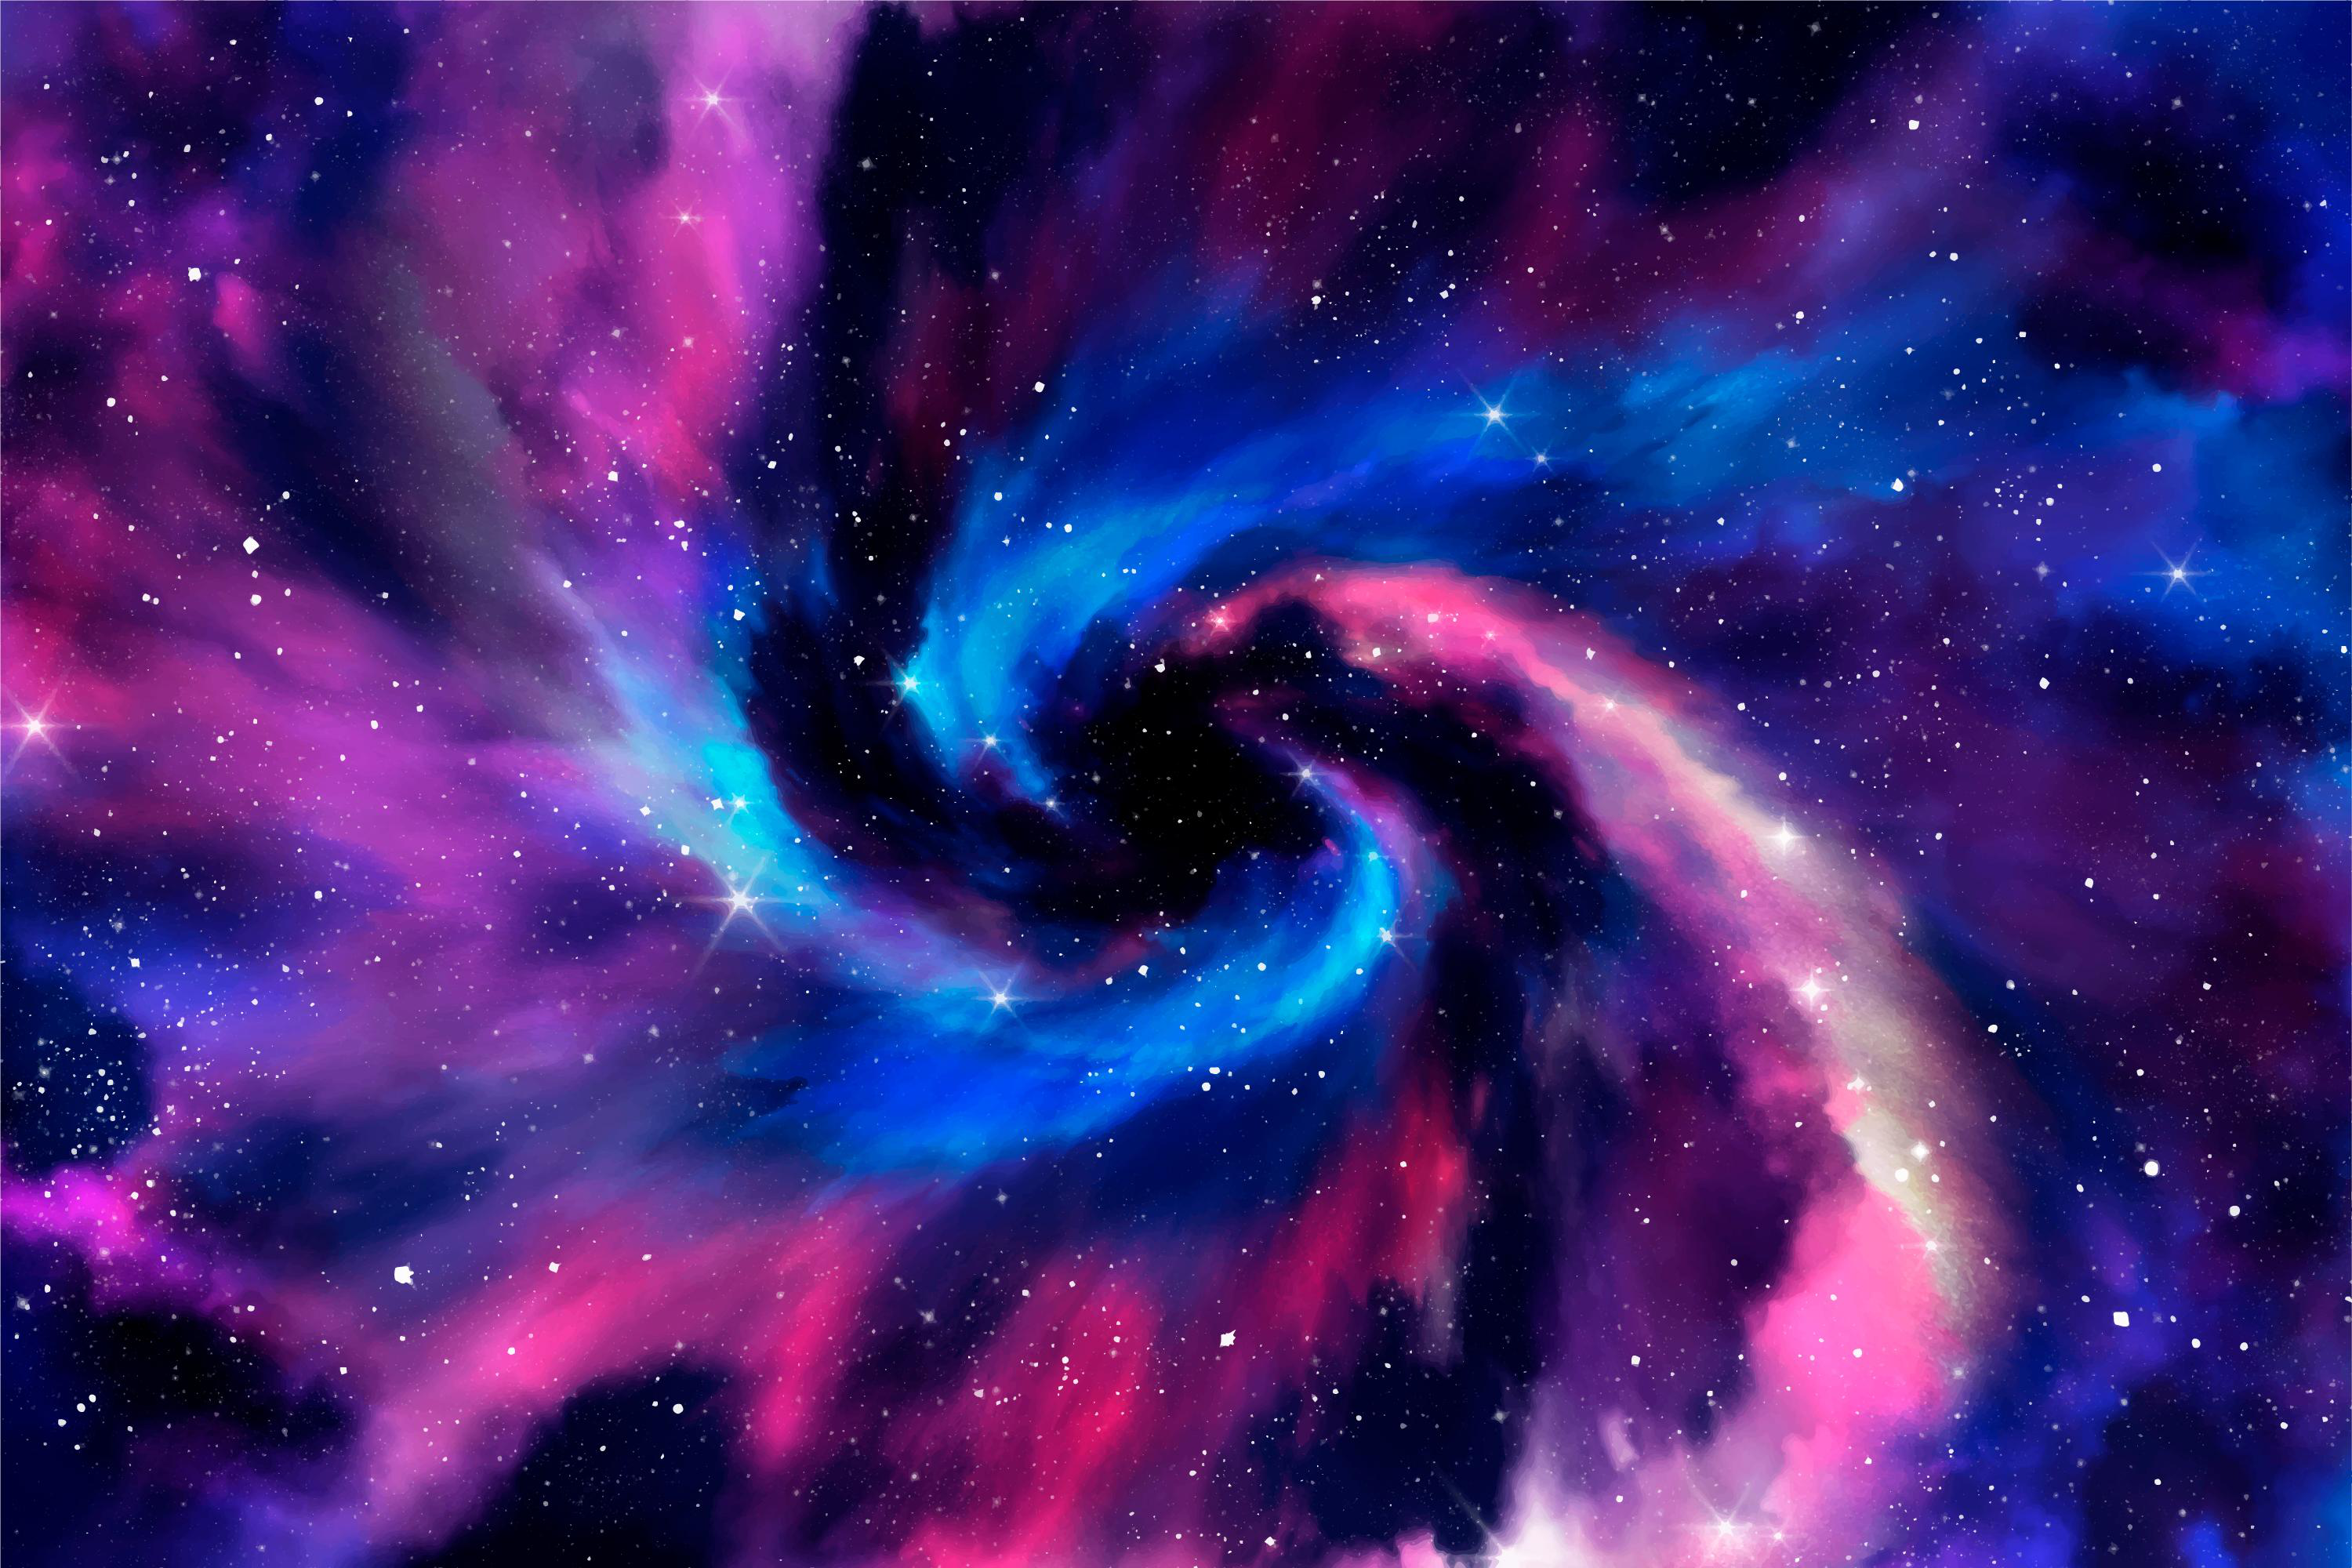
\includegraphics[width=4cm]{../Ch-electrochem/figure1}} node[rotate=90, font=\tiny] at ([yshift=.5cm,xshift=.1cm]a.south east) {\textsuperscript{\textcopyright} PxFuel} ;
%\end{tikzpicture}
%\end{marginfigure}


  \import{../\chapterlabel/files/}{ChapterIntro}
%\begin{marginfigure}%LEARNING GOALS BOX
%\begin{mytcbox}{GOALS}
%\begin{enumerate}[label=\protect\circled{\color{white}\arabic*}]
%\item Identify anodes/cathodes
%\item Calculate cell potentials
%\item Interpret the line notation
%\item Calculate cell potentials of concentration cells
%\item Relate cell potential with $\Delta \text{G}^{\circ}$
%\end{enumerate}
%\end{mytcbox}
%\vspace{1cm}
%\begin{tcolorbox}[enhanced,colback=red!5!white,colframe=black!50!red,boxrule=1pt,
%  arc=0pt,outer arc=0pt,drop heavy lifted shadow]
%\faGears\ 
%  \import{../\chapterlabel/files/}{ChapterDiscussion}
%
%
%\end{tcolorbox}
%\end{marginfigure}%LEARNING GOALS BOX

\section{Introduction to galvanic cells}\import{../\chapterlabel/files/}{SectionIntro-Introduction-to-galvanic-cells}
\sloppy\begin{description}
\item[\docfilehook{Components of a galvanic cell}{ }] 	\import{../\chapterlabel/files/}{Subsection-Introduction-to-galvanic-cells-Components-of-a-galvanic-cell}
\item[\docfilehook{The electrodes: anode and cathode}{ }]\import{../\chapterlabel/files/}{Subsection-Introduction-to-galvanic-cells-The-electrodes:-anode-and-cathode}
\item[\docfilehook{Cell potential}{ }]\import{../\chapterlabel/files/}{Subsection-Introduction-to-galvanic-cells-Cell-potential}
\item[\docfilehook{Role of the salt bridge or the membrane}{ }]\import{../\chapterlabel/files/}{Subsection-Introduction-to-galvanic-cells-Role-of-the-salt-bridge-or-the-membrane}
\item[\docfilehook{A galvanic cell example}{ }]\import{../\chapterlabel/files/}{Subsection-Introduction-to-galvanic-cells-A-galvanic-cell-example}
\import{../\chapterlabel/files/}{Figure-Daniell-cell}
\item[\docfilehook{The potentiometer}{ }] \import{../\chapterlabel/files/}{Subsection-Introduction-to-galvanic-cells-The-potentiometer}
\import{../\chapterlabel/problems/}{SampleProblem1}
\end{description}

\section{Standard reduction potentials}\import{../\chapterlabel/files/}{SectionIntro-Standard-reduction-potentials} 
\sloppy\begin{description}
\item[\docfilehook{Electrode potentials}{ }]\import{../\chapterlabel/files/}{Subsection-Standard-reduction-potentials-Electrode-potentials}
\item[\docfilehook{Standard conditions for reduction potentials}{ }]\import{../\chapterlabel/files/}{Subsection-Standard-reduction-potentials-Standard-conditions-for-reduction-potentials}
\import{../\chapterlabel/files/}{Figure-Batter-hydrogen-electrode}
\item[\docfilehook{Anodes and cathodes}{ }]\import{../\chapterlabel/files/}{Subsection-Standard-reduction-potentials-Anodes-and-cathodes}
\import{../\chapterlabel/problems/}{SampleProblem2}
\end{description}

\import{../\chapterlabel/files/}{Table-redox} 


\section{Redox reactions in galvanic cells}\import{../\chapterlabel/files/}{SectionIntro-Redox-reactions-in-galvanic-cells} 
\sloppy\begin{description}
\item[\docfilehook{Identifying the anodic and cathodic reaction}{ }]\import{../\chapterlabel/files/}{Subsection-Redox-reactions-in-galvanic-cells-Identifying-the-anodic-and-cathodic-reaction}
 \import{../\chapterlabel/files/}{Figure-Gold-Vanadium-galvanic-cell}
  \item[\docfilehook{Cell potential from electrodic voltages}{ }]\import{../\chapterlabel/files/}{Subsection-Redox-reactions-in-galvanic-cells-Cell-potential-from-electrodic-voltages}
   \item[\docfilehook{Electrons flowing}{ }]\import{../\chapterlabel/files/}{Subsection-Redox-reactions-in-galvanic-cells-Electrons-flowing}
 \import{../\chapterlabel/problems/}{SampleProblem3}
\end{description}

\section{Line notation for galvanic cells}\import{../\chapterlabel/files/}{SectionIntro-Line-notation}
  \import{../\chapterlabel/problems/}{SampleProblem4}



\section{Cell potential, Gibbs free energy, and equilibrium constant}\import{../\chapterlabel/files/}{SectionIntro-Cell-potential-and-Gibbs-free-energy}
\sloppy\begin{description}
 \item[\docfilehook{Maximum work given by a galvanic cell}{ }] \import{../\chapterlabel/files/}{Subsection-Maximum-Cell-potential-and-Gibbs-free-energy-work-given-by-a-galvanic-cell}
  \item[\docfilehook{Reduction potentials and Gibbs free energy}{ }] \import{../\chapterlabel/files/}{Subsection-Cell-potential-and-Gibbs-free-energy-Reduction-potentials-and-Gibbs-free-energy}
 \import{../\chapterlabel/problems/}{SampleProblem5}
  \item[\docfilehook{Reduction potentials and equilibrium constant}{ }] \import{../\chapterlabel/files/}{Subsection-Cell-potential-and-Gibbs-free-energy-Reduction-potentials-and-equilibrium-constant}
\end{description}

\section{Electrochemical series: dissolving metals in acid}\import{../\chapterlabel/files/}{SectionIntro-Electrochemical-series}
\sloppy\begin{description}
   \item[\docfilehook{Reducing character}{ }] \import{../\chapterlabel/files/}{Subsection-Electrochemical-series-Reducing-character}
  \import{../\chapterlabel/problems/}{SampleProblem6}
\item[\docfilehook{Can an acid dissolve a metal?}{ }] \import{../\chapterlabel/files/}{Subsection-Electrochemical-series-Can-an-acid-dissolve-a-metal}
\end{description}


\section{Nernst equation}\import{../\chapterlabel/files/}{SectionIntro-Nernst-equation}
\sloppy\begin{description}
   \item[\docfilehook{The Nernst equation applied to an electrode}{ }] \import{../\chapterlabel/files/}{Subsection-Nernst-equation-The-Nernst-equation-applied-to-an-electrode}
   \item[\docfilehook{The Nernst equation applied to a galvanic cell}{ }] \import{../\chapterlabel/files/}{Subsection-Nernst-equation-The-Nernst-equation-applied-to-a-glavanic-cell}
     \import{../\chapterlabel/problems/}{SampleProblem8}
   \item[\docfilehook{The Nernst equation and a drained galvanic cell}{ }] \import{../\chapterlabel/files/}{Subsection-Nernst-equation-The-Nernst-equation-and-a-drained-glavanic-cell}
   \item[\docfilehook{Concentration cells}{ }] \import{../\chapterlabel/files/}{Subsection-Nernst-equation-Concentration-cells}
\import{../\chapterlabel/files/}{Figure-Daniell-concentration-cell}
  \import{../\chapterlabel/problems/}{SampleProblem7}
   \item[\docfilehook{Ion-selective electrodes}{ }] \import{../\chapterlabel/files/}{Subsection-Nernst-equation-Ion-selective-electrodes}
\end{description}
 
 \section{Electrolysis}\import{../\chapterlabel/files/}{SectionIntro-Electrolysis}
\sloppy\begin{description}
    \item[\docfilehook{Galvanic cell vs. electrolytic cell}{ }] \import{../\chapterlabel/files/}{Subsection-Electrolysis-Galvanic-cell-vs.-electrolytic-cell}
\import{../\chapterlabel/files/}{Figure-Daniell-cell-electrolysis}
     \item[\docfilehook{Intensity, charge and time}{ }] \import{../\chapterlabel/files/}{Subsection-Electrolysis-Intensity-charge-and-time}
     \import{../\chapterlabel/problems/}{SampleProblem9}
     \item[\docfilehook{The electrolysis of water}{ }] \import{../\chapterlabel/files/}{Subsection-Electrolysis-The-electrolysis-of-water}
\import{../\chapterlabel/files/}{Figure-Electrolysis-water}\vspace{3cm}
     \item[\docfilehook{Electrolysis and ion mixtures}{ }] \import{../\chapterlabel/files/}{Subsection-Electrolysis-Ion-mixtures}

     \item[\docfilehook{Electrolysis applications}{ }] \import{../\chapterlabel/files/}{Subsection-Electrolysis-Aplications}

\end{description}


 \section{Corrosion}\import{../\chapterlabel/files/}{SectionIntro-Corrosion}
 \section{Batteries}\import{../\chapterlabel/files/}{SectionIntro-batteries}







\checkoddpage\ifoddpage \clearpage\thispagestyle{empty}\mbox{}\clearpage \else  \fi \end{document}

